\documentclass[11pt,a4paper]{ctexart}
\usepackage[margin=2.5cm]{geometry}
\usepackage{amsmath,amssymb,booktabs,graphicx,caption}
\usepackage[hidelinks]{hyperref}
\captionsetup{labelsep=period,font=small}
\graphicspath{{../output/figures/}}
\linespread{1.25}

\title{单边关税、对等报复与贸易条件：\\一个多地区多部门 Armington 模型的数值示范}
\author{贾宁远\\对外经济贸易大学国际经济贸易学院}
\date{2026年10月}

\begin{document}
\maketitle

\begin{center}
\fbox{\parbox{0.9\textwidth}{\small \textbf{示意数据声明：}本文使用示意数据，地区为中性标签 A、B、R，结论仅为机制示范，不得解读为对任何真实国家或真实贸易摩擦的定量评估。}}
\end{center}

\begin{abstract}
本文基于示意数据（中性地区标签 A、B、R），用一个三地区两部门的 Armington 一般均衡模型，考察地区 A 对来自 B 的制造业进口加征 10\% 关税（单边情形），以及 B 对等报复（报复情形）的影响。单边情形下，A 自 B 的制造业进口按出厂价值下降约 36\%，需求转向本地与第三方；B 的相对工资下降约 0.65\%，A 的福利上升约 0.020\%，B 的福利下降约 0.040\%。在 B 对等报复后，A 的福利变为下降约 0.041\%，B 的福利损失缩小到约 0.014\%。在本示意设定下，A 对 B 制造业关税的福利最大化水平在网格上约为 11\%，与 10\% 接近；单边情形下 A 的福利收益在贸易弹性 2 到 12 之间均为正。

\noindent\textbf{关键词：}关税；贸易条件；可计算一般均衡；精确变化法
\end{abstract}

\section{引言}

关税的一般均衡效应包括三条渠道：进口方从出口方价格下降中获得的贸易条件收益、进口方的关税收入，以及消费结构扭曲带来的效率损失。在 Armington (1969) 设定及其更一般的引力模型类中，贸易所得可以由少数充分统计量刻画（Arkolakis, Costinot and Rodríguez-Clare 2012），这使得用精确变化法做关税反事实成为标准做法；Ossa (2014) 用这一类模型量化了关税战与贸易谈判。本文以一个三地区两部门的示意模型展示这些机制，重点是单边关税与对等报复下福利的分解与排序。

本文考察两个情形：S1（单边），A 对来自 B 的制造业（MAN）进口加征 10\% 从价关税；S2（报复），在 S1 基础上，B 对来自 A 的制造业进口加征 10\% 关税。地区 R 在两种情形下都不改变政策。可检验的命题是：P1，S1 中 A 自 B 的制造业进口下降，A 的制造业支出转向本地与 R（贸易转移）；P2，S1 中 B 的相对工资下降，A 获得贸易条件改善。报复情形下各方福利的排序作为待检验问题，不作先验断言。

第 2 节介绍模型、数据与求解，第 3 节报告结果，第 4 节为稳健性，第 5 节总结并讨论局限。

\section{模型、数据与求解}

模型为 Costinot and Rodríguez-Clare (2014) 的多部门、无投入产出联系的 Armington 模型。地区 $j$ 的代表性家庭在部门 $s$ 间为 Cobb-Douglas 偏好，部门支出份额为 $\alpha_j^s$；在部门内对各产地产品为 CES 偏好，贸易弹性为 $\varepsilon_s$。劳动在地区内部门间自由流动，地区间不流动；地区 $j$ 对来自 $i$ 的 $s$ 部门产品征收从价关税 $t_{ij}^s$，收入以总额方式返还本地家庭。

记 $Y_j$ 为地区 $j$ 的产值（劳动收入），$E_j$ 为总支出（含关税），$D_j=E_j-Y_j-T_j$ 为贸易赤字（$T_j$ 为关税收入），$\lambda_{ij}^s$ 为 $j$ 的 $s$ 部门含税支出中来自 $i$ 的份额。带撇号的变量表示反事实水平，加帽变量 $\hat x=x'/x$ 表示反事实相对基期的变化。记 $c_{ij}^s=\hat w_i(1+t_{ij}^{s\prime})/(1+t_{ij}^s)$，反事实支出份额、部门价格指数、总支出与收入出清条件为
\begin{align}
\lambda_{ij}^{s\prime}&=\frac{\lambda_{ij}^s (c_{ij}^s)^{-\varepsilon_s}}{\sum_k\lambda_{kj}^s (c_{kj}^s)^{-\varepsilon_s}},\qquad
\hat P_j^s=\Big[\sum_k\lambda_{kj}^s (c_{kj}^s)^{-\varepsilon_s}\Big]^{-1/\varepsilon_s},\\
E_j'&=\frac{\hat w_jY_j+D_j'}{1-\rho_j},\qquad \rho_j=\sum_s\alpha_j^s\sum_i\frac{t_{ij}^{s\prime}}{1+t_{ij}^{s\prime}}\lambda_{ij}^{s\prime},\\
\hat w_iY_i&=\sum_j\sum_s\frac{\lambda_{ij}^{s\prime}\alpha_j^sE_j'}{1+t_{ij}^{s\prime}},
\end{align}
以世界 GDP 为计价单位。福利以实际吸收的变化度量，
\begin{equation}
\hat W_j=\frac{E_j'/E_j}{\prod_s(\hat P_j^s)^{\alpha_j^s}},\qquad
\ln\hat W_j=\ln\hat w_j+\ln\Big(1+\frac{T_j'}{\hat w_jY_j}\Big)-\sum_s\alpha_j^s\ln\hat P_j^s ,
\end{equation}
右侧三项分别称为工资项、关税收入项与价格指数项（基期无关税、无赤字时严格成立）。求解采用 Dekle, Eaton and Kortum (2008) 的精确变化法。

\paragraph{数据与赤字剔除。} 基期为示意的三地区两部门双边贸易流，基期关税为零。原始数据含贸易赤字；按 Dekle, Eaton and Kortum (2008) 的做法，先求解赤字为零的反事实均衡，以之作为政策实验的基期，从而使结果不依赖于计价单位。贸易弹性取 $\varepsilon=4$（Simonovska and Waugh 2014）。

\paragraph{解的检验。} 剔除赤字后各地区贸易余额的相对误差在 $10^{-15}$ 量级，所有出清方程在解处的残差低于 $10^{-16}$；零冲击时解回到基期。以水平量形式重新表述并求解同一模型，得到的工资与福利与精确变化法相差 $2\times10^{-16}$；分两步加征关税与一步加征的结果一致。检验细节见附录。

\section{结果}

表~\ref{tab:sc} 报告两个情形下各地区的福利、工资、福利分解与部门就业的变化，图~\ref{fig:wd} 为福利分解的图示。

\begin{table}[h]
\centering\small
\caption{两个情形下的主要结果（相对基期，\%；示意数据）。福利为实际吸收变化；工资为名义工资变化；关税收入项与价格指数项为式 (4) 中的分解项（对数近似，×100）；就业为部门就业变化}\label{tab:sc}
\begin{tabular}{llrrrrrr}
\toprule
情形 & 地区 & 福利 & 工资 & 关税收入项 & 价格指数项 & 制造业就业 & 其他部门就业 \\
\midrule
S1 & A & 0.0198 & 0.294 & 0.056 & -0.330 & 0.055 & -0.064 \\
S1 & B & -0.0402 & -0.353 & 0.000 & 0.313 & -0.450 & 0.150 \\
S1 & R & 0.0029 & 0.027 & 0.000 & -0.025 & 0.065 & -0.027 \\
\midrule
S2 & A & -0.0411 & -0.191 & 0.054 & 0.096 & -0.120 & 0.141 \\
S2 & B & -0.0142 & 0.083 & 0.081 & -0.179 & -0.161 & 0.054 \\
S2 & R & 0.0071 & 0.039 & 0.000 & -0.032 & 0.029 & -0.012 \\
\bottomrule
\end{tabular}

\end{table}

\paragraph{单边关税（S1）。} 命题 P1 与 P2 都得到数值支持。A 自 B 的制造业进口按出厂价值下降 35.83\%，自 R 的进口上升 1.78\%，本地制造业销售上升 0.70\%。B 的相对工资（$\hat w_B/\hat w_A$）为 0.9935，即下降约 0.65\%。A 的福利上升 0.0198\%。从分解看，A 的名义工资上升 0.294\%，但由于 A 主要消费本地产品，本地价格随工资同步上升，价格指数项为 $-0.330$ 个百分点，二者相抵后实际工资略降；关税收入项为 0.056 个百分点，抵消实际工资的下降后净福利为正。关税收入之所以能超过扭曲成本，是因为 B 的相对工资下降，关税有一部分由 B 的出口方通过更低的出厂价格承担，这就是贸易条件效应。B 的福利下降 0.0402\%，是工资下降（$-0.353$ 个百分点）被本地价格下降（$+0.313$ 个百分点）部分抵消后的净值。R 的福利略有上升，原因是 A 的进口需求从 B 转向 R，R 的工资略有上升（0.027\%）。

\paragraph{量级。} 福利变化只有百分之零点零几，而 A 自 B 的制造业进口下降了三分之一以上，二者看似不相称。原因在于示意数据中 B 的制造业产品只占 A 总支出的约 0.88\%，关税只影响这一小部分支出。福利变化的量级完全取决于示意的贸易份额，不应外推。

\paragraph{对等报复（S2）。} B 报复后，对 A 制造业产品的需求下降，A 的工资由升转降（$-0.191\%$）；A 的本地价格随之下降，价格指数项转为正值（$+0.096$ 个百分点）；A 仍获得关税收入。净效应是 A 的福利下降 0.0411\%，比单边情形低 0.061 个百分点。B 的工资回升（$+0.083\%$），并获得关税收入（$+0.081$ 个百分点），但价格指数上升（$-0.179$ 个百分点），福利净下降 0.0142\%，比单边情形高 0.026 个百分点。因此，在 A 已经加征 10\% 关税、B 以 10\% 对等报复的设定下，与不报复的 S1 相比，报复改善了 B 的福利。这与关税战文献中“单边的最优反应通常是正关税”的思路定性一致（Ossa 2014），但本文没有计算 B 的最优关税，不能据此推断 10\% 是否接近 B 的最优反应。与自由贸易相比，两国在 S2 中都受损。

\begin{figure}[h]
\centering
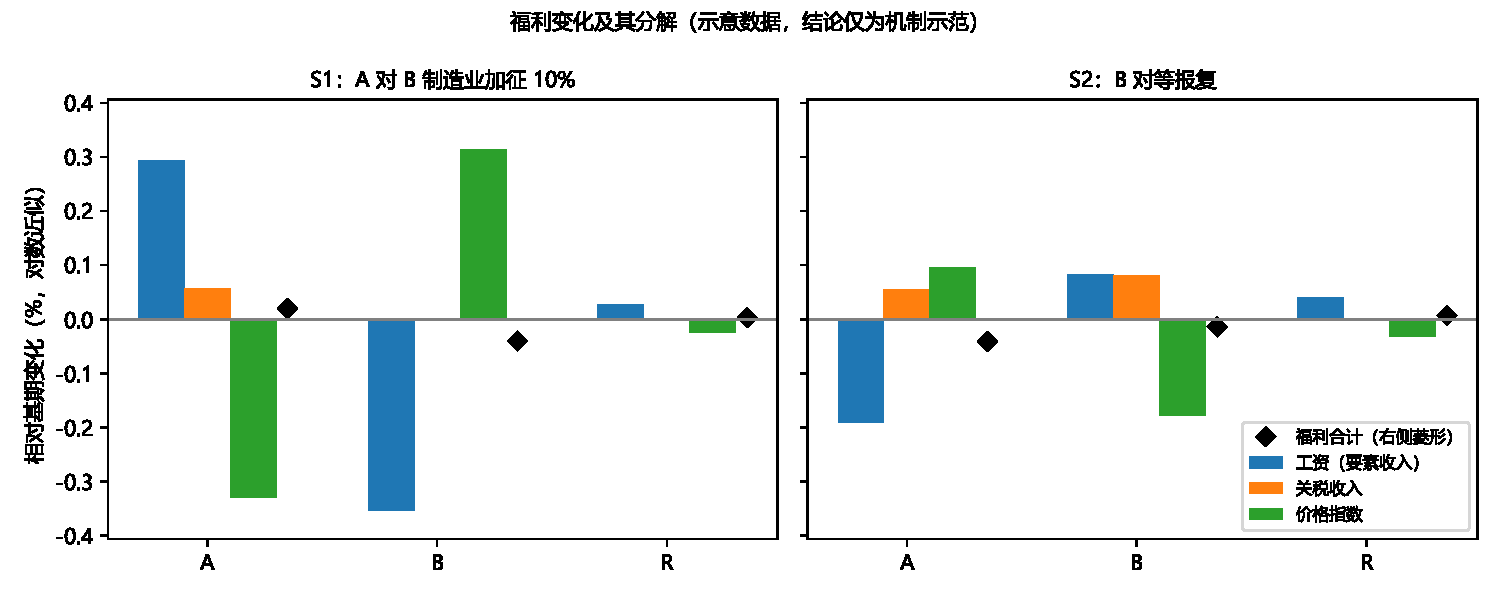
\includegraphics[width=0.98\textwidth]{armington_tariff_welfare_decomposition.pdf}
\caption{福利变化及其分解（示意数据）。左图为 S1（A 对 B 制造业加征 10\%），右图为 S2（B 对等报复）。每个地区的三根柱分别为工资项、关税收入项与价格指数项（相对基期，\%，对数近似），黑色菱形为福利合计，正值表示福利上升}\label{fig:wd}
\end{figure}

\paragraph{数值最优关税。} 图~\ref{fig:ot} 显示，在 B 不报复时，A 的福利随对 B 制造业关税先升后降，在网格上 11\% 处达到最大，福利增益 0.0199\%。最优点附近曲线很平坦：10\% 关税下的福利增益为 0.0198\%，与最优值几乎相同，因此不宜过度解读最优关税的具体数值。

\begin{figure}[h]
\centering
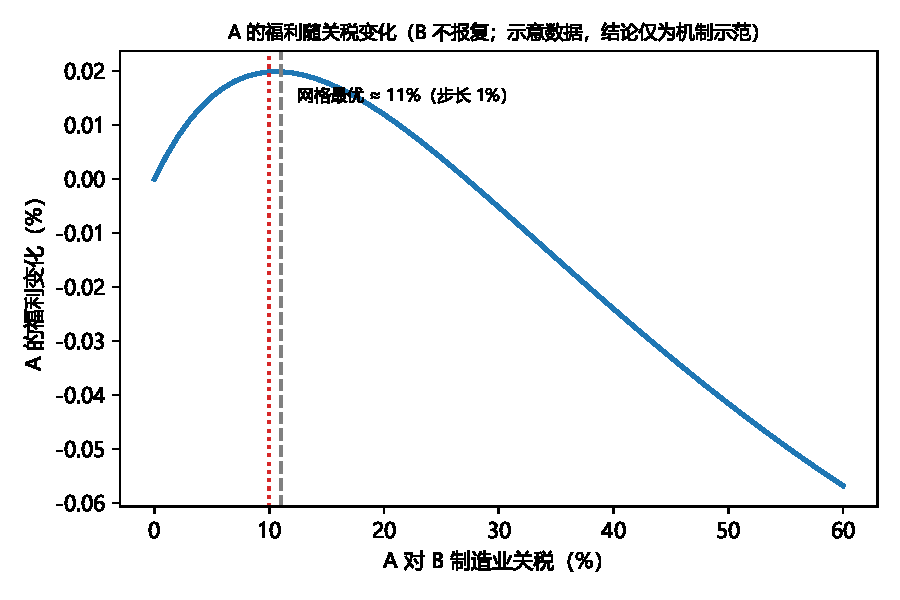
\includegraphics[width=0.6\textwidth]{armington_tariff_optimal_tariff.pdf}
\caption{A 的福利随对 B 制造业关税的变化（B 不报复；示意数据）。横轴为关税率（\%），纵轴为 A 的福利变化（\%）；红色点线为本文情形的 10\%，灰色虚线为网格（步长 1 个百分点）上的福利最大点}\label{fig:ot}
\end{figure}

\section{稳健性}

表~\ref{tab:rob} 报告制造业贸易弹性 $\varepsilon_{MAN}$ 取 2 到 8 时的福利变化，每个弹性值都重新剔除基期赤字。从表中可以看到：第一，单边情形下 A 的福利收益随弹性上升而减小，从 0.0226\% 降至 0.0104\%，因为弹性越高，B 的出口方越容易被替代，越难把关税转嫁给 B；第二，单边情形下 B 的损失随弹性变化不单调；第三，报复情形下 B 的损失随弹性上升而扩大，A 在所有弹性下都受损。以 0.25 为步长把弹性扫描到 12，单边情形下 A 的福利收益始终为正，但在高弹性下已接近零。

\begin{table}[h]
\centering\small
\caption{制造业贸易弹性的稳健性（福利变化，\%；示意数据）}\label{tab:rob}
\begin{tabular}{rrrrr}
\toprule
$\varepsilon_{MAN}$ & S1：A & S1：B & S2：A & S2：B \\
\midrule
2 & 0.0226 & -0.0348 & -0.0406 & -0.0025 \\
3 & 0.0217 & -0.0383 & -0.0408 & -0.0090 \\
4 & 0.0198 & -0.0402 & -0.0411 & -0.0142 \\
6 & 0.0152 & -0.0414 & -0.0420 & -0.0217 \\
8 & 0.0104 & -0.0408 & -0.0427 & -0.0267 \\
\bottomrule
\end{tabular}

\end{table}

\section{总结与局限}

在本示意设定下，单边关税通过贸易条件效应使加税方小幅获益、被加税方受损；对等报复使加税方由获益转为受损，并改善了报复方相对于不报复时的福利；福利最大化关税与 10\% 接近，且最优点附近福利曲线很平坦。

本模型不含投入产出联系、资本积累、内生贸易赤字与策略博弈；基期关税设为零；数据为示意数据。模型中关税通过出口方工资的一般均衡调整产生贸易条件效应；而 2018--2019 年美中关税的实证研究（Amiti, Redding and Weinstein 2019；Fajgelbaum et al. 2020）发现关税几乎完全传递到进口价格。因此本模型的结果只用于说明机制，不能用来解释真实贸易摩擦的福利后果。

\appendix
\section{解的检验}

解的正确性通过以下九类检验确认，均在预设容差（$10^{-12}$ 至 $10^{-9}$）内成立：（1）剔除赤字后各地区贸易余额为零；（2）零冲击时，从偏离基期的初值出发，工资与福利都回到基期；（3）包括冗余方程在内的全部出清方程成立；（4）改用 A 的工资为计价单位时福利不变；（5）水平量表述与精确变化表述的工资与福利一致；（6）分两步加征与一步加征的福利一致；（7）部门就业加总等于地区就业；（8）福利分解各项之和等于福利变化；（9）两种求根方法的解一致。此外，基期数据的会计恒等式与 Arkolakis, Costinot and Rodríguez-Clare (2012) 公式在单部门特例中均成立，但二者按构造必然成立，不能作为解正确性的证据。

\begin{thebibliography}{9}
\bibitem{ard19} Amiti, M., Redding, S. J., \& Weinstein, D. E. (2019). The impact of the 2018 tariffs on prices and welfare. \textit{Journal of Economic Perspectives}, 33(4), 187--210.
\bibitem{acr12} Arkolakis, C., Costinot, A., \& Rodríguez-Clare, A. (2012). New trade models, same old gains? \textit{American Economic Review}, 102(1), 94--130.
\bibitem{a69} Armington, P. S. (1969). A theory of demand for products distinguished by place of production. \textit{IMF Staff Papers}, 16(1), 159--178.
\bibitem{crc14} Costinot, A., \& Rodríguez-Clare, A. (2014). Trade theory with numbers: Quantifying the consequences of globalization. In G. Gopinath, E. Helpman, \& K. Rogoff (Eds.), \textit{Handbook of International Economics}, Vol. 4 (pp. 197--261). Elsevier.
\bibitem{dek08} Dekle, R., Eaton, J., \& Kortum, S. (2008). Global rebalancing with gravity: Measuring the burden of adjustment. \textit{IMF Staff Papers}, 55(3), 511--540.
\bibitem{fg20} Fajgelbaum, P. D., Goldberg, P. K., Kennedy, P. J., \& Khandelwal, A. K. (2020). The return to protectionism. \textit{Quarterly Journal of Economics}, 135(1), 1--55.
\bibitem{o14} Ossa, R. (2014). Trade wars and trade talks with data. \textit{American Economic Review}, 104(12), 4104--4146.
\bibitem{sw14} Simonovska, I., \& Waugh, M. E. (2014). The elasticity of trade: Estimates and evidence. \textit{Journal of International Economics}, 92(1), 34--50.
\end{thebibliography}

\end{document}
